\documentclass[../Main.tex]{subfiles}

\begin{document}

\IfFileExists{NewCommands.tex}       {% Add new commands here.
%
% Use "providecommand" instead of "newcommand" since we
% want to include this file in all subfiles, and if we
% used newcommand it would report the error
% "Command xxx already defined"
%
%
\providecommand{\dmOT}{\Delta m^2_{\rm 12}}
\providecommand{\dmsolar}{\Delta m^2_{\rm solar}}
\providecommand{\dmatm}{\Delta m^2_{\rm atm}}
\providecommand{\dmTT}{\Delta m^2_{\rm atm}}
\providecommand{\dmsq}[1]{\Delta m^{2}_{#1}}
\providecommand{\thatm}{\Delta m^2_{\rm atm}}
\providecommand{\thTT}{\theta_{\rm 23}}
\providecommand{\sinsq}[1]{\sin^{2}(\theta_{#1})}
\providecommand{\sinsqOT}{\sin^{2}(\theta_{\rm 12})}
\providecommand{\sinsqsolar}{\sin^{2}(\theta_{\rm solar})}
\providecommand{\sinsqTT}{\sin^{2}(\theta_{\rm 23})}
\providecommand{\sinsqTwoTT}{\sin^{2}(2\theta_{\rm 23})}
\providecommand{\dcp}{\delta_{\rm CP}}

\providecommand{\gsim}{\gtrsim}
\providecommand{\lsim}{\lesssim}
\providecommand{\Enu}{\rm{E}_\nu}
\providecommand{\Emu}{\rm{E}_\mu}
\providecommand{\Ecasc}{\rm{E}_{\rm casc}}
\providecommand{\Lmu}{\rm{L}_\mu}
\providecommand{\Lnu}{\rm{L}_\nu}
\providecommand{\Thetamu}{\theta_\mu}
\providecommand{\cosThetamu}{\cos{\theta_\mu}}
\providecommand{\cosThetanu}{\cos{\theta_\nu}}
\providecommand{\Thetanu}{\theta_\nu}
\providecommand{\nue}{\nu_{\rm e}}
\providecommand{\numu}{\nu_\mu}
\providecommand{\nutau}{\nu_\tau}

\providecommand{\ket}[1]{|#1\rangle}

\providecommand{\ue}[1]{|U_{e #1}|}
\providecommand{\umu}[1]{|U_{\mu #1}|}
\providecommand{\utau}[1]{|U_{\tau #1}|}
\providecommand{\uesq}[1]{|U_{e #1}|^{2}}
\providecommand{\umusq}[1]{|U_{\mu #1}|^{2}}
\providecommand{\utausq}[1]{|U_{\tau #1}|^{2}}

\providecommand{\Nch}{${\rm N}_{\rm ch}\,$}
\providecommand{\Ndir}{${\rm N}_{\rm dir}\,$}
\providecommand{\Nstr}{${\rm N}_{\rm str}\,$}
\providecommand{\Aeff}{${\rm A}_{\rm eff}\,$}
\providecommand{\Veff}{${\rm V}_{\rm eff}\,$}
\providecommand{\VeffNS}{${\rm V}_{\rm eff}$}

\providecommand{\pe}{$p.e.$ }
}       {}
\IfFileExists{../NewCommands.tex}    {% Add new commands here.
%
% Use "providecommand" instead of "newcommand" since we
% want to include this file in all subfiles, and if we
% used newcommand it would report the error
% "Command xxx already defined"
%
%
\providecommand{\dmOT}{\Delta m^2_{\rm 12}}
\providecommand{\dmsolar}{\Delta m^2_{\rm solar}}
\providecommand{\dmatm}{\Delta m^2_{\rm atm}}
\providecommand{\dmTT}{\Delta m^2_{\rm atm}}
\providecommand{\dmsq}[1]{\Delta m^{2}_{#1}}
\providecommand{\thatm}{\Delta m^2_{\rm atm}}
\providecommand{\thTT}{\theta_{\rm 23}}
\providecommand{\sinsq}[1]{\sin^{2}(\theta_{#1})}
\providecommand{\sinsqOT}{\sin^{2}(\theta_{\rm 12})}
\providecommand{\sinsqsolar}{\sin^{2}(\theta_{\rm solar})}
\providecommand{\sinsqTT}{\sin^{2}(\theta_{\rm 23})}
\providecommand{\sinsqTwoTT}{\sin^{2}(2\theta_{\rm 23})}
\providecommand{\dcp}{\delta_{\rm CP}}

\providecommand{\gsim}{\gtrsim}
\providecommand{\lsim}{\lesssim}
\providecommand{\Enu}{\rm{E}_\nu}
\providecommand{\Emu}{\rm{E}_\mu}
\providecommand{\Ecasc}{\rm{E}_{\rm casc}}
\providecommand{\Lmu}{\rm{L}_\mu}
\providecommand{\Lnu}{\rm{L}_\nu}
\providecommand{\Thetamu}{\theta_\mu}
\providecommand{\cosThetamu}{\cos{\theta_\mu}}
\providecommand{\cosThetanu}{\cos{\theta_\nu}}
\providecommand{\Thetanu}{\theta_\nu}
\providecommand{\nue}{\nu_{\rm e}}
\providecommand{\numu}{\nu_\mu}
\providecommand{\nutau}{\nu_\tau}

\providecommand{\ket}[1]{|#1\rangle}

\providecommand{\ue}[1]{|U_{e #1}|}
\providecommand{\umu}[1]{|U_{\mu #1}|}
\providecommand{\utau}[1]{|U_{\tau #1}|}
\providecommand{\uesq}[1]{|U_{e #1}|^{2}}
\providecommand{\umusq}[1]{|U_{\mu #1}|^{2}}
\providecommand{\utausq}[1]{|U_{\tau #1}|^{2}}

\providecommand{\Nch}{${\rm N}_{\rm ch}\,$}
\providecommand{\Ndir}{${\rm N}_{\rm dir}\,$}
\providecommand{\Nstr}{${\rm N}_{\rm str}\,$}
\providecommand{\Aeff}{${\rm A}_{\rm eff}\,$}
\providecommand{\Veff}{${\rm V}_{\rm eff}\,$}
\providecommand{\VeffNS}{${\rm V}_{\rm eff}$}

\providecommand{\pe}{$p.e.$ }
}    {}
\IfFileExists{../../NewCommands.tex} {% Add new commands here.
%
% Use "providecommand" instead of "newcommand" since we
% want to include this file in all subfiles, and if we
% used newcommand it would report the error
% "Command xxx already defined"
%
%
\providecommand{\dmOT}{\Delta m^2_{\rm 12}}
\providecommand{\dmsolar}{\Delta m^2_{\rm solar}}
\providecommand{\dmatm}{\Delta m^2_{\rm atm}}
\providecommand{\dmTT}{\Delta m^2_{\rm atm}}
\providecommand{\dmsq}[1]{\Delta m^{2}_{#1}}
\providecommand{\thatm}{\Delta m^2_{\rm atm}}
\providecommand{\thTT}{\theta_{\rm 23}}
\providecommand{\sinsq}[1]{\sin^{2}(\theta_{#1})}
\providecommand{\sinsqOT}{\sin^{2}(\theta_{\rm 12})}
\providecommand{\sinsqsolar}{\sin^{2}(\theta_{\rm solar})}
\providecommand{\sinsqTT}{\sin^{2}(\theta_{\rm 23})}
\providecommand{\sinsqTwoTT}{\sin^{2}(2\theta_{\rm 23})}
\providecommand{\dcp}{\delta_{\rm CP}}

\providecommand{\gsim}{\gtrsim}
\providecommand{\lsim}{\lesssim}
\providecommand{\Enu}{\rm{E}_\nu}
\providecommand{\Emu}{\rm{E}_\mu}
\providecommand{\Ecasc}{\rm{E}_{\rm casc}}
\providecommand{\Lmu}{\rm{L}_\mu}
\providecommand{\Lnu}{\rm{L}_\nu}
\providecommand{\Thetamu}{\theta_\mu}
\providecommand{\cosThetamu}{\cos{\theta_\mu}}
\providecommand{\cosThetanu}{\cos{\theta_\nu}}
\providecommand{\Thetanu}{\theta_\nu}
\providecommand{\nue}{\nu_{\rm e}}
\providecommand{\numu}{\nu_\mu}
\providecommand{\nutau}{\nu_\tau}

\providecommand{\ket}[1]{|#1\rangle}

\providecommand{\ue}[1]{|U_{e #1}|}
\providecommand{\umu}[1]{|U_{\mu #1}|}
\providecommand{\utau}[1]{|U_{\tau #1}|}
\providecommand{\uesq}[1]{|U_{e #1}|^{2}}
\providecommand{\umusq}[1]{|U_{\mu #1}|^{2}}
\providecommand{\utausq}[1]{|U_{\tau #1}|^{2}}

\providecommand{\Nch}{${\rm N}_{\rm ch}\,$}
\providecommand{\Ndir}{${\rm N}_{\rm dir}\,$}
\providecommand{\Nstr}{${\rm N}_{\rm str}\,$}
\providecommand{\Aeff}{${\rm A}_{\rm eff}\,$}
\providecommand{\Veff}{${\rm V}_{\rm eff}\,$}
\providecommand{\VeffNS}{${\rm V}_{\rm eff}$}

\providecommand{\pe}{$p.e.$ }
} {}


\graphicspath{{figures/}{PhysicsDetectorSimulation/figures/}}


\section{Physics and Detector Simulation}\label{sec:PhysDetSim}

The generation of simulated data for the IceCube and DeepCore detectors is broken down into three distinct components.  The first component is the generation of the neutrinos themselves as well as their interactions within the nucleus.  Once these interaction products are outside of the nucleus, their movement and light production is handled by a particle propagator.  The final component required is a light propagator which is responsible only for tracking the photons produced and determining the final hits produced at the detector.

\subsection{Neutrino Signal Generation}\label{sec:neutSignal}

For the majority of the past, generation of ``high energy'' neutrino signal for the IceCube neutrino telescope has used the NuGen event generator, which is based on ANIS \cite{Gazizov:2004va}.  This method has proven to be reliable for neutrino energies above roughly 100 GeV, however the requirement of simulating DeepCore events (lowering the energy to roughly 10 GeV) necessitated another option.  The generator chosen is GENIE \cite{Andreopoulos:2009rq} which has been previously used primarily by the accelerator-based neutrino community to accurately model few-GeV interactions.  The method of simulation also differs because GENIE conducts a simulation of the interaction between the neutrino and the nucleon and produces a list of the particles exiting from the interaction vertex.  In addition to this simulation, intranuclear effects are included in the simulation and the generation of the daughter particles.  All neutrino interaction channels are modeled by the GENIE code, although particularly at energies higher than the few GeV scale, the majority of the events arise from deep inelastic scattering (DIS).

In order to incorporate the GENIE neutrino generator into the IceCube software framework, a wrapper was written which can be used within the existing code.  This wrapper takes as inputs ranges of the desired location and direction as well as the energy spectrum for the generated neutrinos.  Following production, the neutrinos are provided with new weights (reweighted) based on the energy spectrum with which they were thrown and the desired atmospheric spectrum.  Currently the code allows for weights to be generated in relation to several different models \cite{Honda2015}, \cite{Bartol2004}, or \cite{Fluka2003}.  In this manner spectra can be used which are specific to the location of IceCube at the South Pole as the geomagnetic effects of the Earth have been included in the calculation, as well as the asymmetry in the flux as a function of azimuth and zenith.

In addition to the ability to weight the neutrinos to an atmospheric spectrum, the use of the simulation in this manner allows for the inclusion of various systematics and their effect on the final event rate.  In particular, GENIE uses detailed modeling of the physics of the neutrino interaction, the parameters of which can therefore be studied as changes in the weight of the event.  These uncertainty parameters are specific to the interaction type, which in DeepCore consists primarily of deep inelastic scattering (DIS), baryon resonance production (RES), and quasi-elastic (QEL) interactions.  The uncertainties associated with these types are discussed separately.

The majority of the events considered in the DeepCore detector are DIS events.  The GENIE simulation code includes a model provided by Bodek and Yang \cite{BodekYang} which accounts for higher twist and corrections to the target mass.  The parameters specifically used in this analysis for the DIS events deal with the twist parameterization (AhtBY and BhtBY) and the correction to the u valence quark in the GRV98 PDF (CV1uBY and CV2uBY).  The resonance production events are generated using the Rein-Sehgal model \cite{ReinSehgal} and have the uncertainties associated with the axial mass for charged current (MaCCRES) and neutral current (MaNCRES) interactions included.


%To improve performance, neutrino interactions simulated outside of a
%cylinder of 200~m radius and 500~m height, centered on PINGU, are
%discarded at the outset.  Because the atmospheric muon veto is
%extremely effective at rejecting particles originating outside of the
%PINGU fiducial volume, the reduction in neutrino rate at the analysis
%level introduced by this approximation should be negligible.


\subsection{Neutrino Background Generation}\label{sec:background}

The backgrounds which affect the DeepCore detector are primarily cosmic ray muons which penetrate into the DeepCore detector.  These are predominantly removed by using the IceCube strings surrounding DeepCore as a veto, and thereby rejecting any hit which has light generated in these strings.  Since the flux of muons produced by cosmic ray showers is roughly $10^6$ times the atmospheric neutrino flux, it is computationally expensive to generate a full set representative of these muons.  This issue has two separate solutions.  The time intensive solution involves the use of Corsika \cite{Heck} to generate the cosmic ray air showers and then to propagate the resultant muons into the detector.  Similar to the neutrino signal generation, these events can be weighted to represent a full neutrino flux without generating the full sample size.  A more expedient solution is to use a generator specifically designed to inject muons at specific angles into the detector.  These muons can then be used to determine the 

%Computational resource limitations do not permit generation of event
%samples comparable to the expected atmospheric muon rates, so we rely
%primarily on the demonstrated muon rejection performance of the
%IceCube DeepCore detector to support our estimates of muon background
%rates.  Because the outermost DeepCore instrumentation, which is
%deployed in the extremely clear ice below about 2100 m depth, will be
%used to reinforce the muon veto provided by the main IceCube detector,
%this estimate should be strongly conservative.  Accordingly, our
%neutrino efficiencies are calculated by applying slightly modified
%DeepCore event selection routines to our simulated neutrino events,
%and the atmospheric muon samples produced for PINGU are primarily
%intended to confirm that these event selections behave as expected.
%
%Two methods were used to produce samples of the atmospheric muon
%background.  The first utilized full Corsika simulation of air showers
%produced by cosmic rays incident on the upper atmosphere, tracking the
%muons produced in such air showers to the PINGU detector.  The second,
%known as the ``muon gun,'' parametrizes the angular and energy
%distributions of the muons produced in the Corsika simulations and
%injected muons from a half-sphere extending just outside the IceCube
%detector volume.   


\subsection{Direct Photon Propagation}\label{sec:photonPropagation}

The relativistic particles produced at a GENIE neutrino interaction
vertex were tracked by GEANT4 until they, and any daughter particles
produced, fell below the Cherenkov threshold.  All of the Cherenkov
photons produced were stored for later propagation through the ice by
a separate simulation program.  This provides a more detailed model of
the light emission from the neutrino interaction vertex than the
standard IceCube tools, which relies instead on parametrized
descriptions of prototypical hadronic and electromagnetc showers.
Atmospheric muons traveling through the detector were modeled using
the standard IceCube particle propagator MMC~\cite{Chirkin:2004hz},
instead of GEANT4.

\subsection{Light Propagation}
\label{sec:}

Once the relativistic particles were propagated through the detector
volume by GEANT4 or MMC, the Cherenkov photons produced were tracked
by the IceCube software tool ``clsim.''  This is a parallelized,
GPU-based software package which permits full treatment of photon
propagation throughout the extremely large volume occupied by IceCube.
The depth-dependent optical properties of the Antarctic ice have been
extensively studied by the IceCube Collaboration, and the full details
of this optical model~\cite{Aartsen:2013rt} were included.  At each
propagation step, photon scattering is modeled by numerical
approximations to the Mie scattering function, as developed and tuned
by IceCube.

\subsection{Detector Response}\label{sec:detResponse}

The main optical elements of the planned PINGU DOMs are identical to
those used in DeepCore, so the detector response modeling of the DOMs
was used without modification (except that an average calibration
function was used for each DOM, rather than the individualized DOM
models used in IceCube simulations).   Recent studies of dark noise in
IceCube have shown that there is a significant non-Poissonian
component to the DOM noise, possibly arising from scintillation in the
pressure glass or the PMT glass at very low temperatures; this effect
was included in the detector simulation.

Although the digitization electronics used in PINGU will differ from
the IceCube and DeepCore design, no modifications were made to the
simulation software.  The dynamic range of PINGU may be slightly
narrower, but given the much lower energy range of the neutrinos of
interest, saturation of the PINGU electronics should be
rare for events of interest.  The timing resolution of the PINGU
electronics will be similar to that of IceCube, so the photon timing and
pulse resolution should be similar.  The PINGU electronics, based on
fast ADCs, will provide this timing resolution over the full event
time range without deadtime, whereas the IceCube electronics
occasionally need to fall back on a slower FADC with coarser timing
resolution.

In IceCube and DeepCore, data rates from individual DOMs are reduced
by imposition of a local coincidence in hardware.  If neighboring DOMs
also detect light, a full data record is transmitted to the surface;
otherwise, only a brief summary record is sent.  No dedicated local
coincidence circuitry is planned for PINGU, but we anticipate that
faster FADCs, onboard photoelectron pulse extraction in FPGAs, and
string-level software coincidence logic at the surface will allow us
to fit PINGU data within the available cable bandwidth.  Again, to the
extent that the PINGU hardware differs from the model used in
simulation, the additional flexibility in software-based coincidence
logic will only improve PINGU performance over the model used in
simulation.  We therefore have a high degree of confidence in our
simulation of PINGU.

The trigger rate in DeepCore is quite low, demanding only
three close-neighbor DOMs with locally-coincident hits within a time
window of a 2.5 microseconds.  Although this threshold may not be
feasible given the much higher number of DOMs in PINGU, very few
simulated neutrino events near the trigger threshold survive the
relatively strict event selection applied to neutrino events used in
the performance studies presented here.  We anticipate that the
inclusion of spatial, as well as timing, information into the PINGU
trigger will permit use of trigger algorithms which would record all
of the events used in these studies.


%\begin{figure}
%\centering
%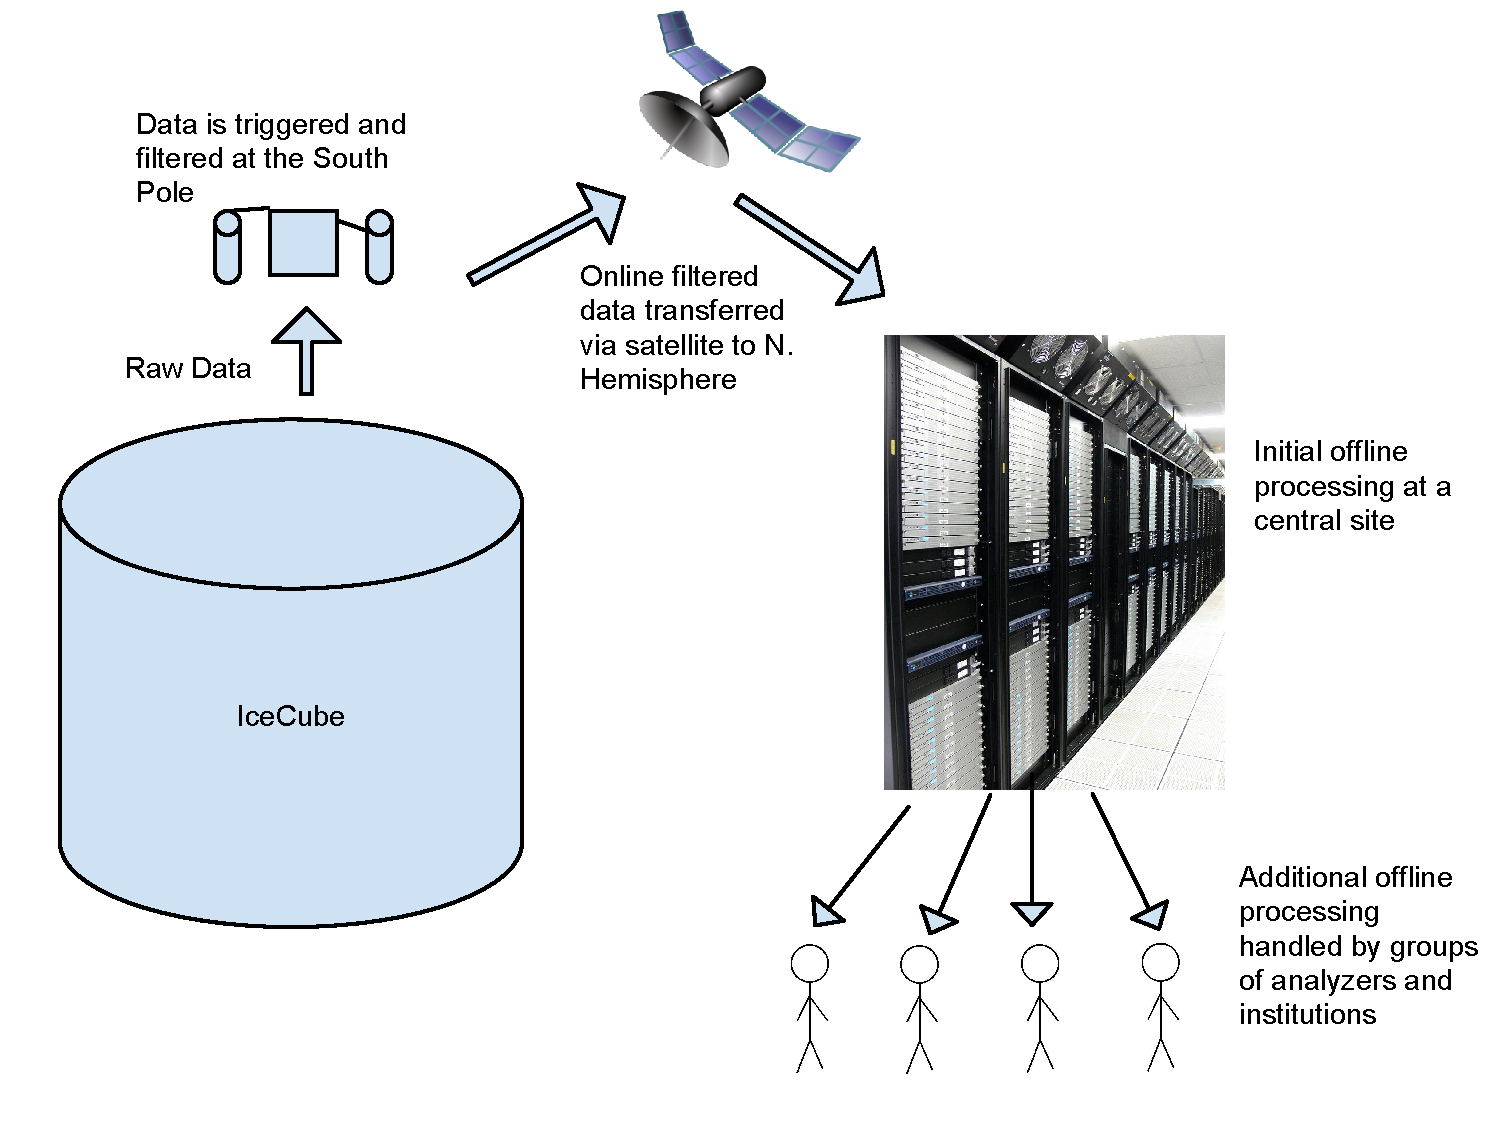
\includegraphics[scale=0.4]{Online_IceCube_data_processing_flow_chart.pdf}
%\caption{\label{fig:DataFlowChart} Should we include, an obviously
%  nicer, flow chart of data collection? More simple? Redundant because
%it'll be in the IceCube Detector paper?}
%\end{figure}

\end{document}
